\documentclass[12pt]{article}

\usepackage{pablo-devoir}
\usepackage[a5paper]{geometry}

\pagestyle{empty}

\title{(In)Équations}
\date{15 octobre}
\classe{2\up{des}14}
\dsnum{DM 2}

\begin{document}

\maketitle
\begin{exercice}[Développement --- Factorisation]
  Soient les trois fonctions suivantes :
  \begin{itemize}[$\bullet$]
    \item $f(x)=x^2-4x-5$
    \item $f_1(x)=\left( x+1 \right)\left( x-5 \right)$
    \item $f_2(x)=\left( x-2 \right)^2-9$
  \end{itemize}
  
  \begin{enumerate}
    \item Montrer que les trois formes $f$, $f_1$ et $f_2$ sont égales.
    \item Calculer $f(0)$ et $f(5)$.
    \item En utilisant la forme appropriée, résoudre les équations suivantes :

      \begin{inparaenum}[(a)]
        \item $f(x)=0$
        \item $f(x)=-9$
        \item $f(x)=-5$
      \end{inparaenum}
  \end{enumerate}
\end{exercice}

\begin{exercice}[Inéquations]
  Résoudre les inéquations suivantes, et présenter le résultat sous forme d'intervalles.
  \begin{multicols}{2}
    \begin{enumerate}[(a)]
      \item $4x-7\leq 10x+8$
      \item $9+3x<-2$
      \item $1+x<2$ et $x+3\geq 0$
      \item $2\left( x+1 \right)<-1+2x$
    \end{enumerate}
\end{multicols}
\end{exercice}

\begin{exercice}[Problème ouvert]~
  \begin{multicols}{2}
  Pour quelles valeurs de $x$ est-il possible de construire le triangle ci-contre ?

  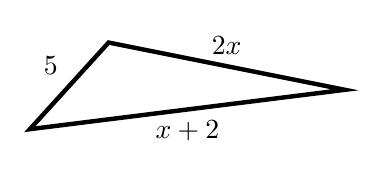
\begin{tikzpicture}[ultra thick]
    \draw (0,-0.4) -- (3,-1) node[midway,above]{$2x$} -- (-1,-1.5) node[midway,below]{$x+2$}-- cycle node[midway,above left]{$5$};
\end{tikzpicture}

\end{multicols}
\end{exercice}

\end{document}
